\documentclass[aspectratio=169]{beamer}
\usetheme{Madrid}
\usecolortheme{default}

% Packages
\usepackage{graphicx}
\usepackage{booktabs}
\usepackage{biblatex}
\addbibresource{references.bib}
\usepackage{algorithmic}
\usepackage{algorithm}

\setbeamertemplate{navigation symbols}{}


% \usepackage[backend=biber,style=alphabetic]{biblatex}
% \addbibresource{references.bib}

\setbeamertemplate{footline}{
    \leavevmode%
    \hbox{%
        \begin{beamercolorbox}[wd=.33\paperwidth,ht=2.5ex,dp=1ex,leftskip=1em]{author in head/foot}%
            \textbf{MNIT Jaipur}
        \end{beamercolorbox}%
        \begin{beamercolorbox}[wd=.33\paperwidth,ht=2.5ex,dp=1ex,center]{title in head/foot}%
            Minor Project
        \end{beamercolorbox}%
        \begin{beamercolorbox}[wd=.33\paperwidth,ht=2.5ex,dp=1ex,rightskip=1em]{date in head/foot}%
            4th December, 2025 \hfill \insertframenumber/\inserttotalframenumber
        \end{beamercolorbox}%
    }%
    \vskip0pt%
}


% Title and Author Information
% \title[Precision Agriculture]{ Hybrid geo-science based NIA optimisation models for Crop rotation modelling in Precision Agriculture for Rajasthan}

\title[Using Landsat 8/9 temporal datasets for Crop Recommendation in Rajasthan: An enhanced approach for Precision Agriculture]{Using Landsat 8/9 temporal datasets for Crop Recommendation in Rajasthan: An enhanced approach for Precision Agriculture}

\author{\textbf{\textcolor{blue}{Aadhya Joshi}} (2022UCP1326) \\ \textbf{\textcolor{blue}{Nandini}} (2022UCP1341)}

\institute{
    Malaviya National Institute of Technology, Jaipur \\ % Institute Name
    Department of Computer Science and Engineering % Department Name
    \\
    
}
\date{4th December, 2025}
\vspace{2mm}


\begin{document}

% Slide 1: Title Slide
\begin{frame}
    \titlepage
    \vspace{-0.7cm}  % Reduce vertical space for better fitting
    \begin{center}
        
\includegraphics[width=0.08\textwidth]{Mnit_logo.png}\\  % Resize logo
        \small{Under the supervision of}\\  % Reduce font size for the guide name
        \textbf{\textcolor{blue} {Dr. Lavika Goel}}, Assistant Professor % Bold and smaller font size for the guide's name
    \end{center}
\end{frame}







\begin{frame}{Outline}

    \begin{itemize}
        \item Introduction
        \item Motivation
        \item Problem Statement
        \item Literature Review
        \item Research Gaps
        \item Objective
        \item Proposed Methodology
        \item Conclusion and Future Scope
        \item Acknowledgements
        \item References
    \end{itemize}
    
\end{frame}


% \begin{itemize}
%     \item Rajasthan’s agriculture faces challenges such as erratic rainfall, poor soil health, and limited water resources.
%     \item To address this, we propose an Advanced Intelligent Crop Recommendation System that uses machine learning, remote sensing, and hybrid optimization algorithms to suggest the most suitable crops based on soil, climate, and market conditions.
%     \item This system aims to boost yield, promote sustainable practices, and support data-driven decision making for farmers.
    
% \end{itemize}

\begin{frame}{Introduction}
\begin{itemize}
    \item Rajasthan’s agriculture faces persistent challenges such as erratic rainfall, degrading soil health, and limited water resources.
    
    \item An existing Crop Recommendation System has been developed using machine learning and remote-sensing features, but it is currently trained only on \textbf{2021–22 agricultural data}.
    
    \item We have \textbf{studied, analysed, and re-implemented} its data curation workflow and training algorithms to understand the methodology, datasets, and limitations.
    
    \item We have initiated \textbf{dataset expansion} to include \textbf{multiple subsequent years} to capture seasonal variability and improve model generalization.
\end{itemize}
\end{frame}


\begin{frame}{Motivation}
\begin{itemize}
    \item Precision agriculture requires multi-year, seasonally diverse data to capture real variations in climate, soil health, and crop patterns.

    \item The existing Crop Recommendation System relies mainly on \textbf{2021–22 data}, which limits its ability to reflect annual fluctuations in rainfall, temperature, irrigation, and extreme weather events.

    \item Crop suitability and productivity are highly time-dependent, and single-year datasets fail to represent trends, anomalies, and shifting agricultural conditions across Rajasthan.

    \item Curating a \textbf{comprehensive multi-year dataset}—including satellite features, weather parameters, and ground data—forms the essential foundation for future accurate crop modelling.

    \item Strengthening the dataset with \textbf{temporal depth} will help improve model performance and generalization, and reduce overfitting.
\end{itemize}
\end{frame}


\begin{frame}{Problem Statement }

Traditional crop recommendation systems struggle to handle high-dimensional and multispectral remote-sensing data, especially when extended across multiple years. Most existing systems rely on limited single-year datasets, failing to capture temporal variability in climate, soil conditions, and crop behavior. There is a need for robust, scalable models that integrate \textbf{multi-year environmental, soil, and satellite data} for accurate and adaptable crop recommendation. This study supports the development of future temporally rich, precision-focused crop recommendation systems for Rajasthan.

\end{frame}

    % \item Develop novel hybrid Nature-Inspired Algorithms (NIAs) by combining:
    % \begin{itemize}
    %     \item GSA–ALO, iEACOP–BBO, Hippo–Walrus, GSA–HGS
    % \end{itemize}
    
    % \item Apply hybrid NIAs to optimize ANN weights and biases for accurate crop recommendation.

    % \item Select key features (e.g., NDVI, soil moisture) using hybrid NIAs to reduce complexity and improve model performance.

    % \item Evaluate proposed NIAs against baseline optimizers using Landsat-8/9 and soil-climate data of Rajasthan (rabi \& kharif).

\begin{frame}{Literature Review I}
\begin{table}[ht]
    \centering
    \caption{Related Work}
    \tiny
    \begin{tabular}{|p{0.3in} | p{0.78in}| p{0.68in}| p{1.2in}|p{1.35in}|}
    \hline
    \textbf{Year} & \textbf{Author} &  \textbf{Paper} & \textbf{Contributions} & \textbf{Research Gaps} \\
    \hline
    \vspace{1mm}
  2025 & Salunke et al. \cite{salunke2025deep} & Deep Learning based Hybrid Approach for Crop Recommendation on the basis of Soil, Environment and Market Commodity Data & \begin{itemize}
    \item Proposes a hybrid ensemble \textbf{DCNN-LSTM} model achieving 98.7\% accuracy.
    \item Novel integration of \textbf{market commodity data} to recommend alternative, profitable crops.
\end{itemize}  & \begin{itemize}
    \item Difficulty in \textbf{harmonizing diverse datasets} (soil, weather, market) due to varying formats and scales.
    \item \textbf{Insufficient data granularity} affects the precision of local-level predictions.
\end{itemize}  \\
    \hline
    \vspace{1mm}
  2025 & Hadeeqa et al. \cite{hadeeqa2025incorporating} & Incorporating soil information with machine learning for crop recommendation to improve agricultural output &  \begin{itemize}
    \item Proposes the \textbf{RFXG} (Random Forest and XGBoost) ensemble, achieving 98\% accuracy.
    \item Uses essential soil nutrients (N, P, K, pH) and climate data for 22 crops.
\end{itemize} & \begin{itemize}
    \item \textbf{Limited exploration of multimodal data} integration (e.g., satellite/drone imagery) to improve robustness.
    \item Continuous need for more \textbf{accurate and comprehensive data} to fully capture soil and climate dynamics.
\end{itemize} \\
    \hline
    \end{tabular}
\end{table}
\end{frame}

\begin{frame}{Literature Review II}
\begin{table}[ht]
    \centering
    \tiny
    \begin{tabular}{|p{0.3in} | p{0.78in}| p{0.68in}| p{1.2in}|p{1.35in}|}
    \hline
    \textbf{Year} & \textbf{Author} &  \textbf{Paper} & \textbf{Contributions} & \textbf{Research Gaps} \\
    \hline
    \vspace{1mm}
  2024 & Senapaty, Murali Krishna, Abhishek Ray, and Neelamadhab Padhy \cite{senapaty2024decision} & A decision support system for crop recommendation using machine learning classification algorithms  & \begin{itemize}
    \item Evaluates 13 machine learning classifiers to improve crop recommendation using state specific data.
    \item SMOTE with the SGDC classifier achieves the best accuracy.
\end{itemize}  & \begin{itemize}
    \item Limited incorporation of explainable AI techniques
    \item Insufficient exploration on larger datasets.
\end{itemize}  \\
    \hline
    \vspace{1mm}
%    2024 & Buttar, Preetpal Kaur \cite{buttar2024satellite} & Satellite imagery analysis for crop type segmentation using U-net architecture  & \begin{itemize}
%        \item Comparative machine learning applied.
%    \end{itemize}  & \begin{itemize}
%     \item High parameter count in U-Net (31M) poses computational challenges.
%     \item Limited geographic validation.
%     \item Simplistic loss functions constrain model performance.
% \end{itemize}  \\
2024 & Buttar et al. \cite{buttar2024semantic} & Semantic segmentation of satellite images for crop type identification in smallholder farms &  \begin{itemize}
    \item Crop type detection on small land parcels.
    \item Propose an attention based encoder-decoder network, CropNet.
    \item Improves mean IoU by 2.5\% .
\end{itemize} & \begin{itemize}
    \item Used temporal data as channels, which is inappropriate.
    \item Use of recurrent  units for time series data.
    \item Huge number of parameters required.

\end{itemize} \\
    \hline
    \end{tabular}
    % \label{IDS}
\end{table}
\end{frame}

% \begin{frame}{Literature Review III}
% \begin{table}[ht]
%     \centering
%     \tiny
%     \begin{tabular}{|p{0.3in} | p{0.78in}| p{0.68in}| p{1.2in}|p{1.35in}|}
%     \hline
%     \textbf{Year} & \textbf{Author} &  \textbf{Paper} & \textbf{Contributions} & \textbf{Research Gaps}  \\
%     \hline
%    2024 &  Pawan et al. \cite{unknown} & An effective approach for crop recommendation using features of specific locations and seasons to maximize crop yield production using machine learning  & \begin{itemize} 
%     \item Leveraged a dataset of 2200 samples with 20 features and 22 classes of crops.
%     \item Random forest outperformed others with 98.18\% accuracy.
%     \item Handled uncertainties, noise, and missing values.
% \end{itemize}   & \begin{itemize}
%     \item Lack of user centric features and not sustainable. 
%     \item It is tested only on small dataset.
% \end{itemize} \\
%     \hline

%     2023 &  Gopi, PSS and Karthikeyan, M \cite{gopi2023intelligent} &  Intelligent crop recommendation with yield prediction using dragonfly algorithm based deep learning model  & \begin{itemize}
%     \item Dragonfly algorithm with deep neural network (DNN) model. 
%     \item Cascaded recurrent neural network (CRNN) model.
% \end{itemize} & \begin{itemize}
%     \item Labelled data is required for training of all models. \item Converges faster due to backpropagation
% \end{itemize} \\
%         \hline
%     \end{tabular}
% \end{table}
% \end{frame}

% \begin{frame}{Literature Review IV}
%     \centering
%     \tiny
%     \begin{tabular}{|p{0.3in} | p{0.78in}| p{0.68in}| p{1.2in}|p{1.35in}|}
%     \hline
%     \textbf{Year} & \textbf{Author} &  \textbf{Paper} & \textbf{Contributions} & \textbf{Research Gaps} \\
% %         \hline
% %  2024 & Jia, Zhaohong et al. \cite{jia2024improved} & An improved crop yield prediction using CNN-BiLSTM model with attention mechanism  &  \begin{itemize}
% %     \item A CNN-BiLSTM model with attention mechanism is proposed.
% %     \item BiLSTM outperforms traditional LSTM in yield prediction. 
% %     \item It shows superior prediction accuracy compared to existing methods.
% % \end{itemize}  & \begin{itemize}
% %     \item Lack of long-term yield forecasting approaches.
% %     \item Limited development of user-friendly interfaces for farmers.
% %     \item Insufficient exploration of advanced attention mechanisms to model temporal feature relationships
% % \end{itemize} \\
%         \hline
% 2023 & Kiruthika S, Karthika D \cite{kiruthika2023iot} & IOT-based professional crop recommendation system using a weight-based long-term memory approach  &  \begin{itemize}
%     \item Utilizes IDCSO and WLSTM for improved predictions. 
%     \item Farmers receive instant crop recommendations based on input parameters.
% \end{itemize} & \begin{itemize}
%     \item Integration of additional data sources, such as real-time weather data, soil health metrics.
%     \item Could focus on sustainability and environmental impact.
% \end{itemize} \\
%        \hline
%  2023 & Sathya S, SU RamPrakash et al. \cite{sathya2023season} & Season and production based crop recommendation system for agricultural data using machine learning techniques  &  \begin{itemize}
%      \item Proposes a machine learning-based crop recommendation system with a focus on precision agriculture, real-time data integration, and sustainable practices tailored to the Indian agricultural context.
%  \end{itemize} & \begin{itemize}
%      \item Lack of real-time decision support systems and limited integration of diverse data sources such as satellite imagery, soil health metrics, and socio-economic factors.
%  \end{itemize} \\
% \hline
       
%     \end{tabular}
    
%     % \label{IDS}
% \end{frame}


% \begin{frame}{Literature Review IV}
%     \centering
%     \tiny
%     \begin{tabular}{|p{0.3in} | p{0.78in}| p{0.68in}| p{1.2in}|p{1.35in}|}
%     \hline
%     \textbf{Year} & \textbf{Author} &  \textbf{Paper} & \textbf{Contributions} & \textbf{Research Gaps} \\
%   %       \hline
%   % 2023 &  Mala DJ, Basak S, Reynold A \cite{mala2023intellifarmassist} & Intellifarmassit - a novel machine learning integrated genetic algorithm based optimal crop recommendation system  &  \begin{itemize}
%   %     \item Genetic algorithm is used with Machine learning to give more optimized crop recommendation.
%   % \end{itemize} & \begin{itemize}
%   %     \item Precision due to efficient GA is good but improper balance between exploration and exploitation.
%   % \end{itemize}  \\
        
%         \hline

       
%     \end{tabular}
    
%     % \label{IDS}
% \end{frame}


 % 2023 &  Jayanthi B et al. \cite{jayanthi2023coimbatore} & Crop recommendation system for identifying the better yielding crops using hybrid evolutionary algorithm SS-NMRA (2023) &  \begin{itemize}
 %     \item Introduces the hybrid SS-NMRA model achieving a high F1-score of 0.93, providing both single and multi-crop recommendations to enhance yield and maximize farmer profitability. 
 % \end{itemize} & \begin{itemize}
 %     \item Existing models lack sustainability, use limited feature sets, and leave room for the development of more effective hybrid optimization algorithms.
 % \end{itemize} \\
 %        \hline

\begin{frame}{Research Gaps}
\begin{itemize}
    \item \textbf{Limited Temporal Dataset:} Reliance on single-year data prevents capturing yearly climatic and agricultural variability.

    \item \textbf{Scalability Issues:} Models trained on small datasets fail to generalize across diverse agro-climatic zones.

    \item \textbf{Weak Feature Selection:} Current methods struggle to identify key spatial, soil, and weather features.

    \item \textbf{Poor GIS–ML Integration:} Limited fusion of remote-sensing indices with soil–climate data restricts spatial precision.
\end{itemize}
\end{frame}

\begin{frame}{Objectives}
\begin{itemize}
    \item \textbf{Study and re-implement the existing Crop Recommendation System} (2021–22): reproduce its data-curation pipeline and training procedures to validate results and document limitations.
    \item \textbf{Apply existing classification algorithms and models} to curated dataset to quantify performance gaps, failure modes, and sources of error in current ML approaches.
    \item \textbf{Scale and evaluate:} Expand the dataset to subsequent years and both seasons (Rabi \& Kharif), benchmark the new (NIA) optimizer integrated approach against baseline ML approaches, and define future paths for deployment and continual dataset growth.
\end{itemize}
\end{frame}


\begin{frame}{Proposed Methodology}

\begin{figure}
    \centering
    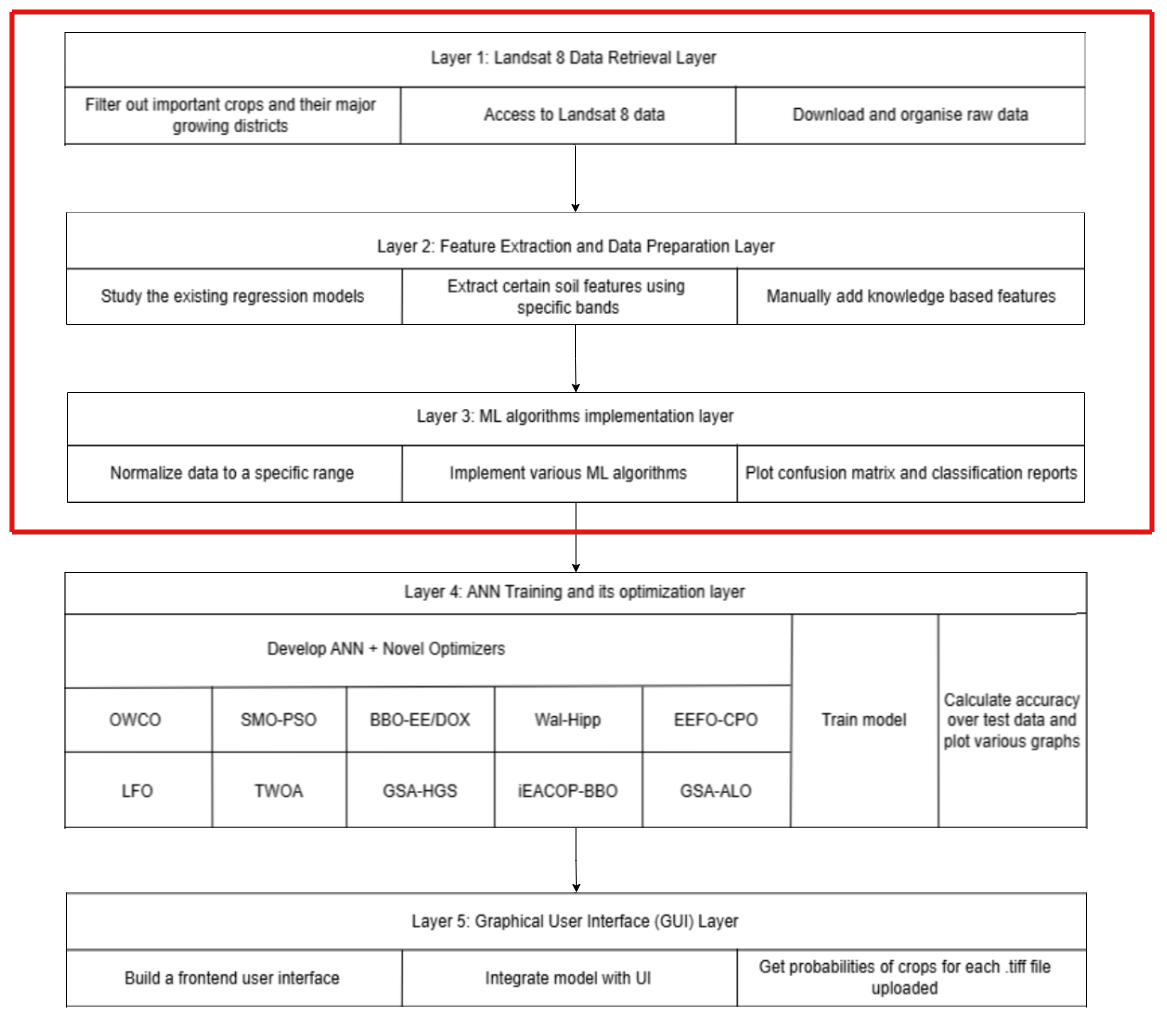
\includegraphics[height=0.42\textwidth,keepaspectratio]{Layered_Architecture.png}
    \caption{Layered Architecture}
    % \label{fig:enter-label}
\end{figure}
\end{frame}

% \begin{frame}{Proposed Methodology II}
% \begin{itemize}
%     \item Developed and implemented four novel hybrid Nature-Inspired Optimization Algorithms:
%     \begin{itemize}
%         \item A hybrid of the Gravitational Search Algorithm (GSA) \cite{rashedi2009gsa} and the Ant Lion Optimization Algorithm \cite{assiri2020ant}
%         \item A hybrid of the Improve Evolutionary Algorithm for Complex Optimization Problem (iEACOP) \cite{tangherloni2024modified}and the Biogeography Based Optimization Algorithm (BBO) \cite{marouani2024enhanced}
%         \item A hybrid of the Hippopotamus Optimization Algorithm (HOA) \cite{amiri2024hippopotamus} and the Walrus Optimization Algorithm (WOA)\cite{han2024walrus}.
%         \item A hybrid of the Gravitational Search Algorithm (GSA) and the Hunger Games Search (HGS) algorithm\cite{yang2021hunger}.

%     \end{itemize}
%     \item All hybrids have shown promising performance in enhancing the accuracy and convergence of the ANN model.
    
% \end{itemize}
% \end{frame}

\begin{frame}{Layer 1: Landsat 8 Data Retrieval Layer}
Landsat 8/9 Level-2 satellite images for 2021–22 were downloaded from USGS EarthExplorer (24 scenes), with 8 surface reflectance bands and surface temperature values. 
\begin{figure}
    \centering
    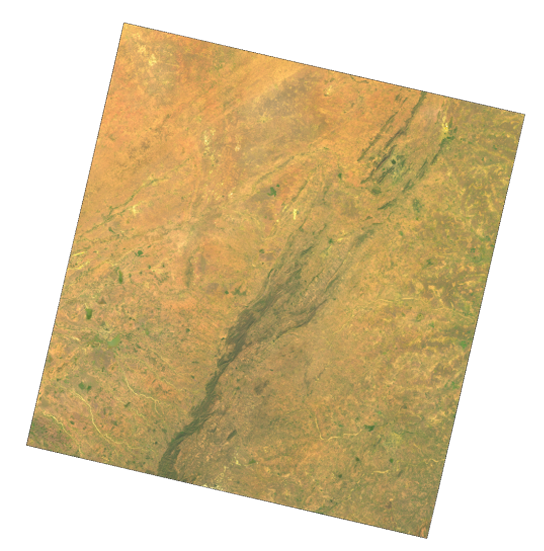
\includegraphics[width=0.3\linewidth]{images/landsat_image_RGB.png}
    \caption{A composite of Landsat red, green and blue bands of a scene with
 path-row 148-042, taken on Nov 9, 2021.}
    \label{fig:placeholder}
\end{figure}
\end{frame}

\begin{frame}{Bands of Landsat-8/9}
    \begin{figure}
        \centering
        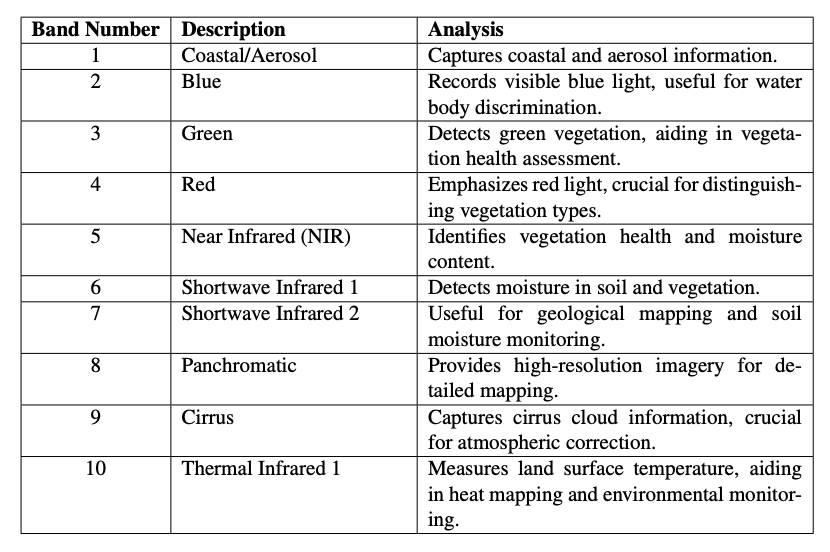
\includegraphics[width=0.6\linewidth]{images/bands.png}
        \caption{Bands used to extract soil characteristics}
        \label{fig:enter-label}
    \end{figure}
\end{frame}

\begin{frame}{Processing Statistical Department Crop Data}
    Village-level area-under-cultivation data for around 10,000 villages was obtained directly from the Department of Statistics, Rajasthan, to improve the spatial resolution of crop mapping. \\
    \begin{figure}
        \centering
        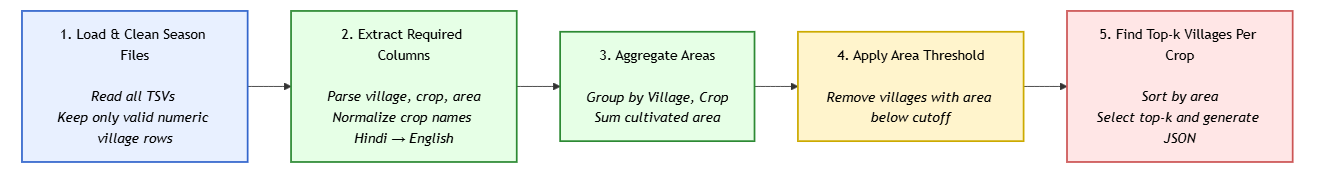
\includegraphics[scale=0.4]{images/flowchart_layer1.png}
        \caption{Village Selection Process}
        \label{fig:placeholder}
    \end{figure}
    \vspace{-2mm}
    \begin{figure}
        \centering
        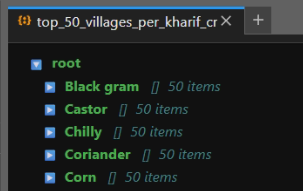
\includegraphics[scale=0.45]{images/top_50_villages_per_crop_2.png}
        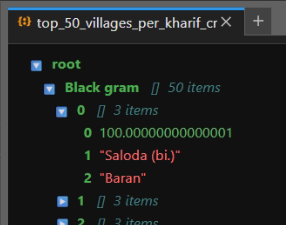
\includegraphics[scale=0.4]{images/top_50_villages_per_crop.png}
        \caption{JSON file for crop-to-village mapping}
        \label{fig:placeholder}
    \end{figure}
    
\end{frame}

\begin{frame}{Layer 2: Feature Extraction and Data Preparation Layer}
Preliminary Data acquired:
    \begin{itemize}
        \item \textbf{Crop Masks:} Google Earth Engine Dynamic World.(In figure: Nov 2021 Crop mask for entire Rajasthan)
        \begin{figure}
            \centering
            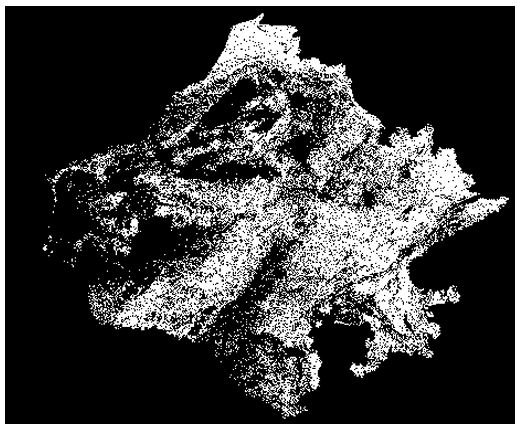
\includegraphics[width=0.2\linewidth]{images/cropmask_2021.png}
            \label{fig:placeholder}
        \end{figure}
        \item \textbf{Boundaries:} Administrative shapefiles from ArcGIS Hub.
        \item \textbf{Weather Data:} Rainfall, temperature, humidity from Open Meteo.
    \end{itemize}
\vspace{3mm}
Dataset Generation Pipeline:
\begin{figure}
    \centering
    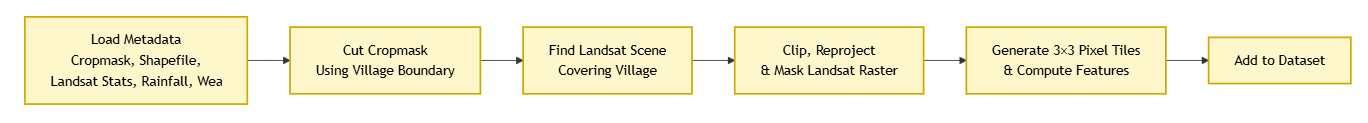
\includegraphics[scale=0.4]{images/flowchart_layer2_1.png}
    \label{fig:placeholder}
\end{figure}
\end{frame}

\begin{frame}{Dataset Generation I}
    A. PREPARE METADATA \& LOAD REQUIRED FILES: \\
    Load crop mask for a season (Kharif/Rabi), village boundary shapefiles, Landsat footprint polygons, Landsat image metadata, rainfall and weather tables \\
    \vspace{5mm}
    B. EXTRACT VILLAGE CROP MASK \& BOUNDARY:
    \begin{figure}
        \centering
        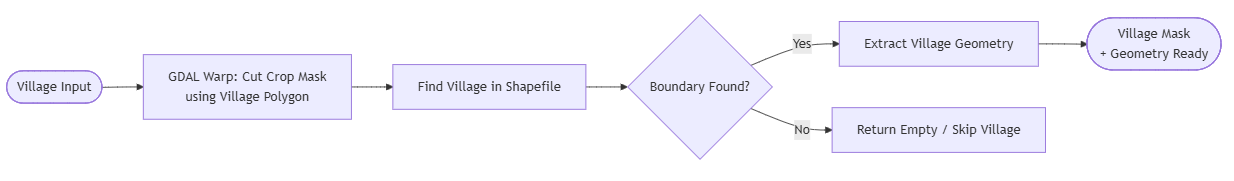
\includegraphics[scale=0.45]{images/flowchart_layer2_2.png}
        \label{fig:placeholder}
    \end{figure}
    
\end{frame}

\begin{frame}{Dataset Generation II}
    C. SELECT LANDSAT SCENE CONTAINING THE VILLAGE:
    \begin{figure}
        \centering
        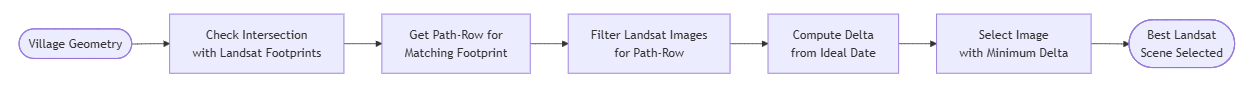
\includegraphics[scale=0.45]{images/flowchart_layer2_3.png}
        \label{fig:placeholder}
    \end{figure}

    D. CLIP, RE-PROJECT \& MASK LANDSAT IMAGE:
    \begin{figure}
        \centering
        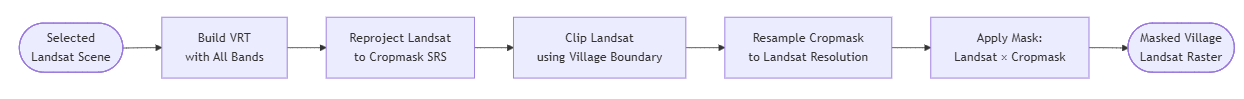
\includegraphics[scale=0.45]{images/flowchart_layer2_4.png}
        \label{fig:placeholder}
    \end{figure}

    \begin{figure}
        \centering
        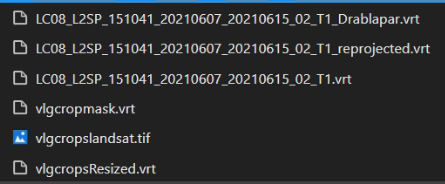
\includegraphics[width=0.3\linewidth]{images/vrt_files_generated.png}
        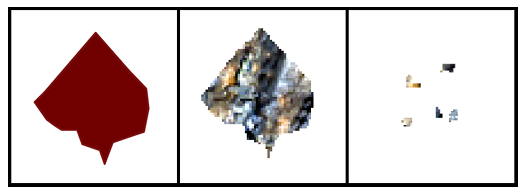
\includegraphics[width=0.35\linewidth]{images/landsat_crop_mask.png}
        \caption{Vector boundary mask for Shivpura Ghata,when
 applied to landsat images gives all pixels of the village.
 These pixels are then subjected to a cropland mask to obtain
 cropland pixels in ShivpuraGhata.}
        \label{fig:placeholder}
    \end{figure}
\end{frame}

\begin{frame}{Dataset Generation III}
    E. GENERATE 3X3 TILES AND COMPUTE FEATURES:
    \vspace{0.2cm}

    % \begin{columns}[t]
    %     % Column 1
    %     \begin{column}[t]{0.3\textwidth}
    %         \centering
    %         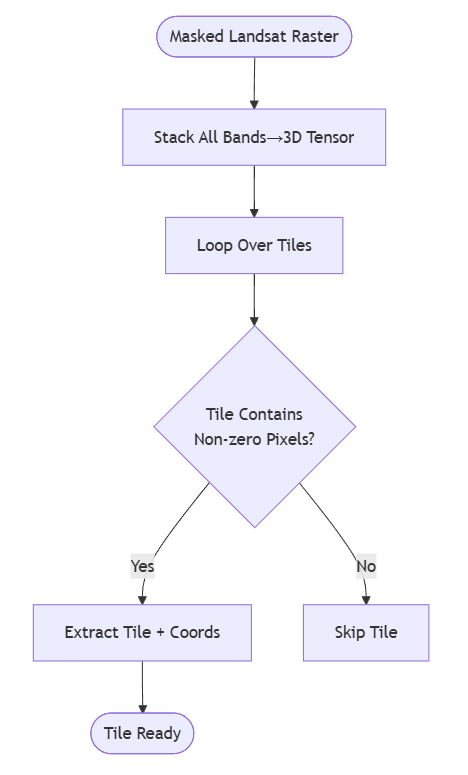
\includegraphics[scale=0.3]{images/flowchart_layer2_5.png}
    %     \end{column}

    %     % Column 2
    %     \begin{column}[t]{0.3\textwidth}
    %         \left
    %         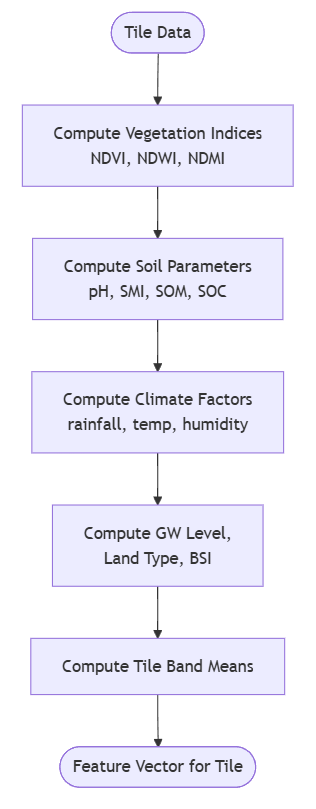
\includegraphics[scale=0.3]{images/flowchart_layer2_6.png}
    %     \end{column}

    %     % Column 3
    %     \begin{column}[t]{0.4\textwidth}
    %             \left
    %             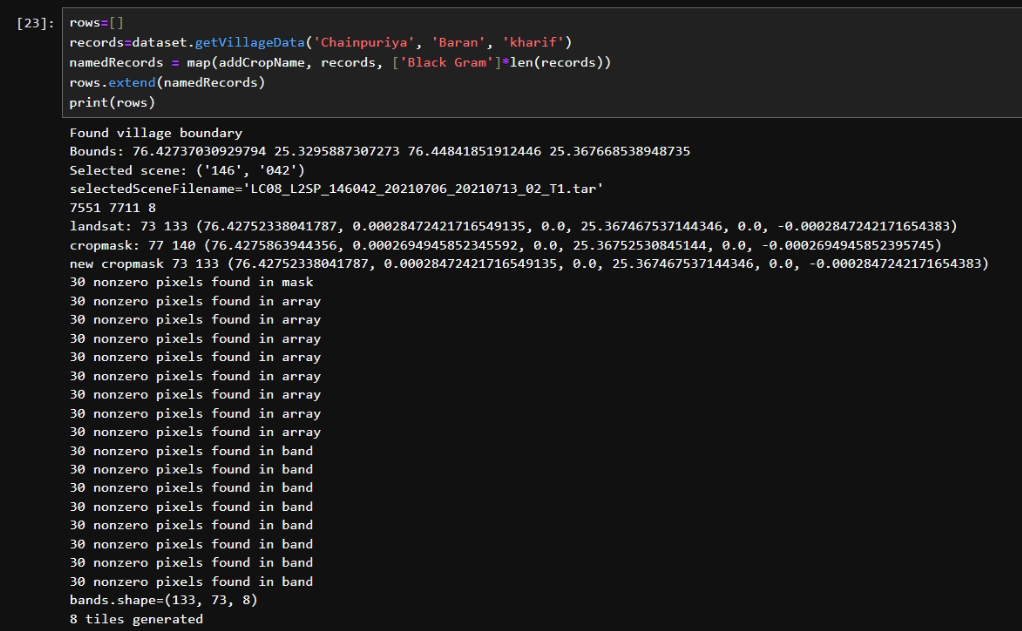
\includegraphics[width=0.9\linewidth]{images/one_village_results.png}
    %     \end{column}
    % \end{columns}
    \begin{minipage}{\textwidth}
        \centering
        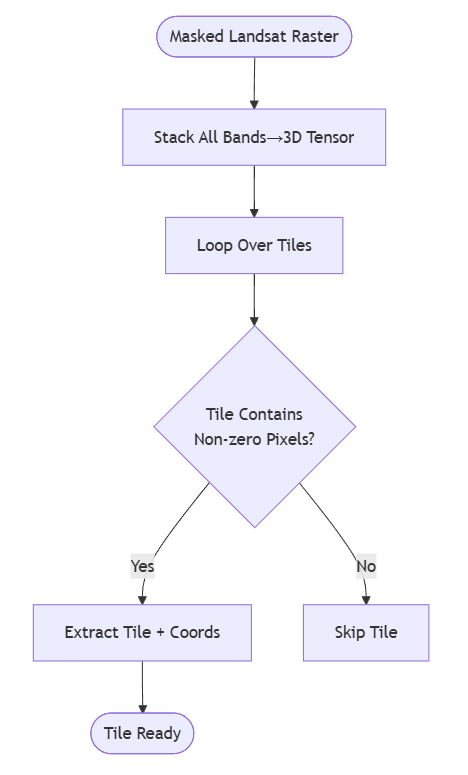
\includegraphics[scale=0.3]{images/flowchart_layer2_5.png}
        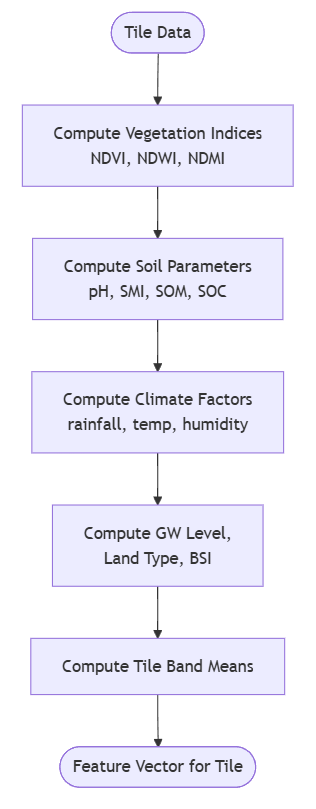
\includegraphics[scale=0.3]{images/flowchart_layer2_6.png}
        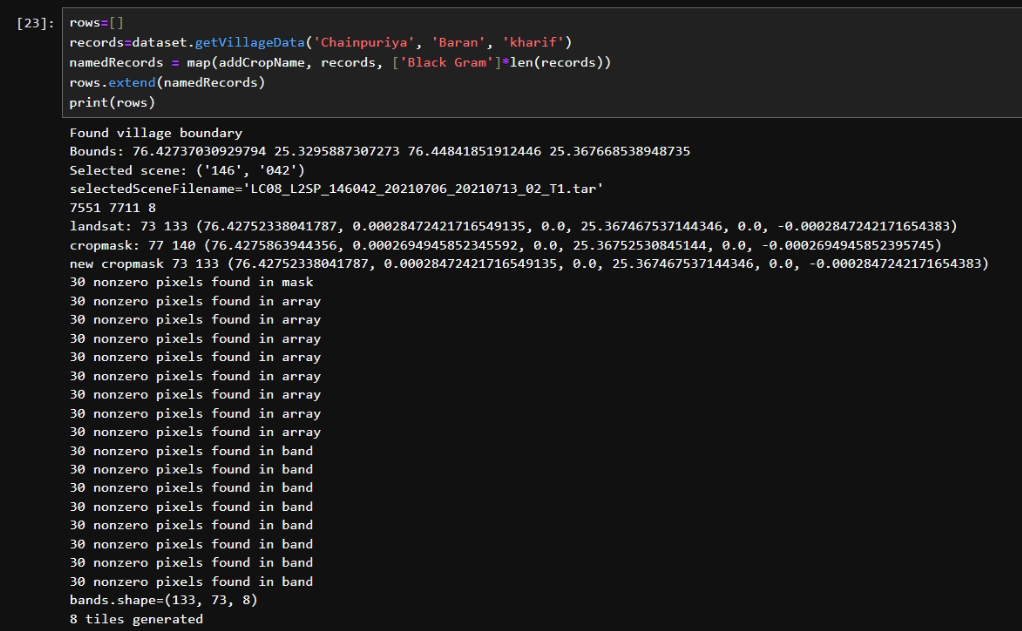
\includegraphics[scale=0.27]{images/one_village_results.png}     
    \end{minipage}
\end{frame}


% -----------------------------------------------------------
\begin{frame}{Dataset Summary}
\begin{itemize}
    \item \textbf{Weather parameters added:} rainfall, min/max temperature, humidity.
    \item \textbf{Crops:} 13 Rabi crops and 16 Kharif crops.
    \item \textbf{Rows:} 52,127 (Rabi), 71,119 (Kharif).
    \item \textbf{Features per row:} 20 engineered features + 8 mean reflectance values.
\end{itemize}
\vspace{2mm}
\centering
\begin{minipage}{0.4\textwidth}
        \centering
        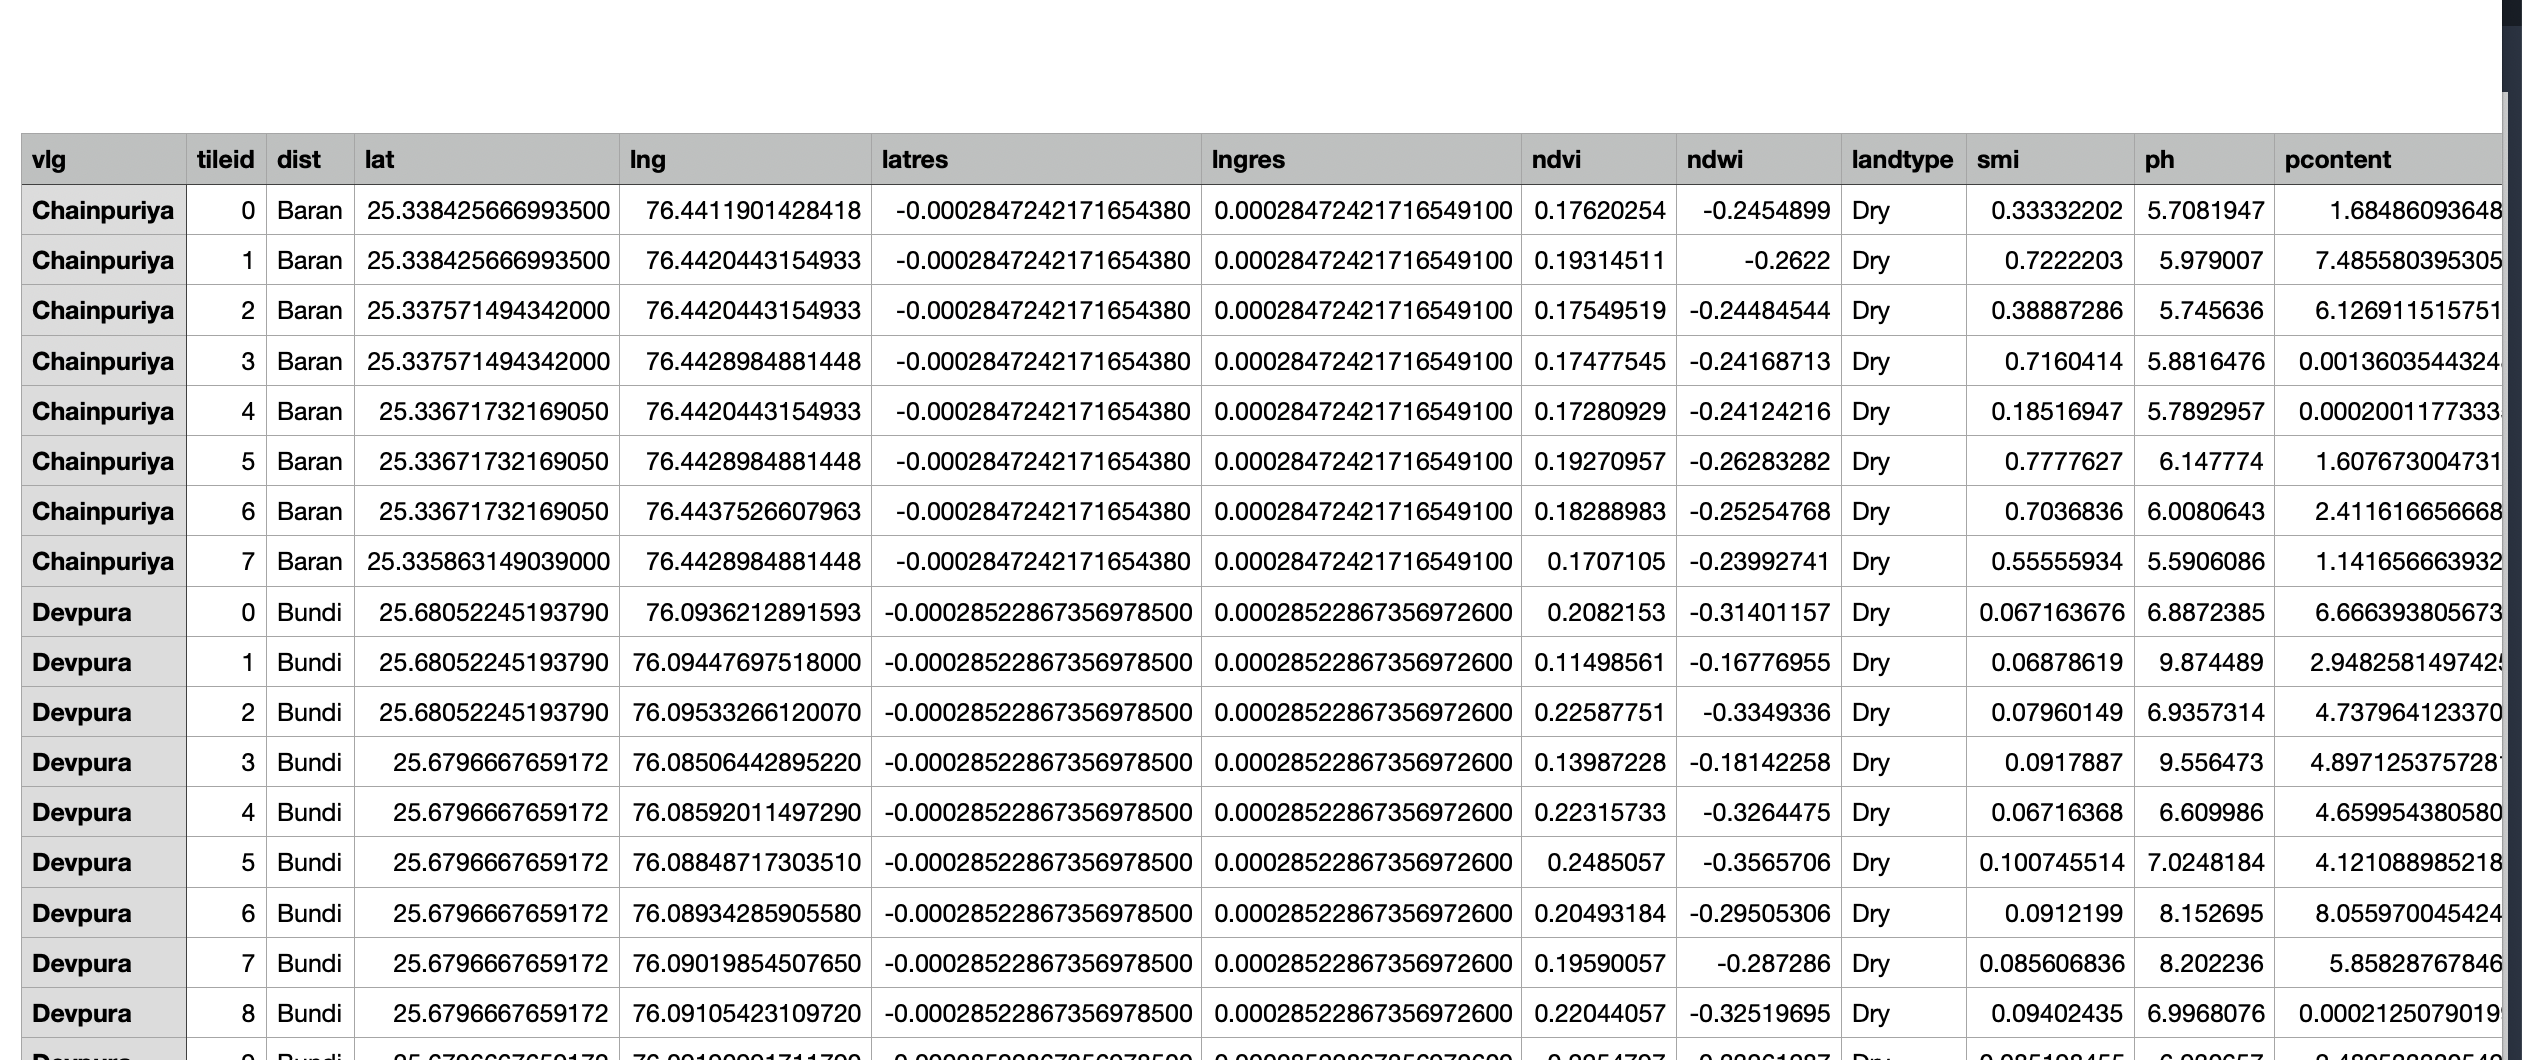
\includegraphics[width=\textwidth]{kharif_dataset.png}  % Replace with your image file
        \caption{Kharif Dataset}
    \end{minipage}
    \begin{minipage}{0.4\textwidth}
        \centering
        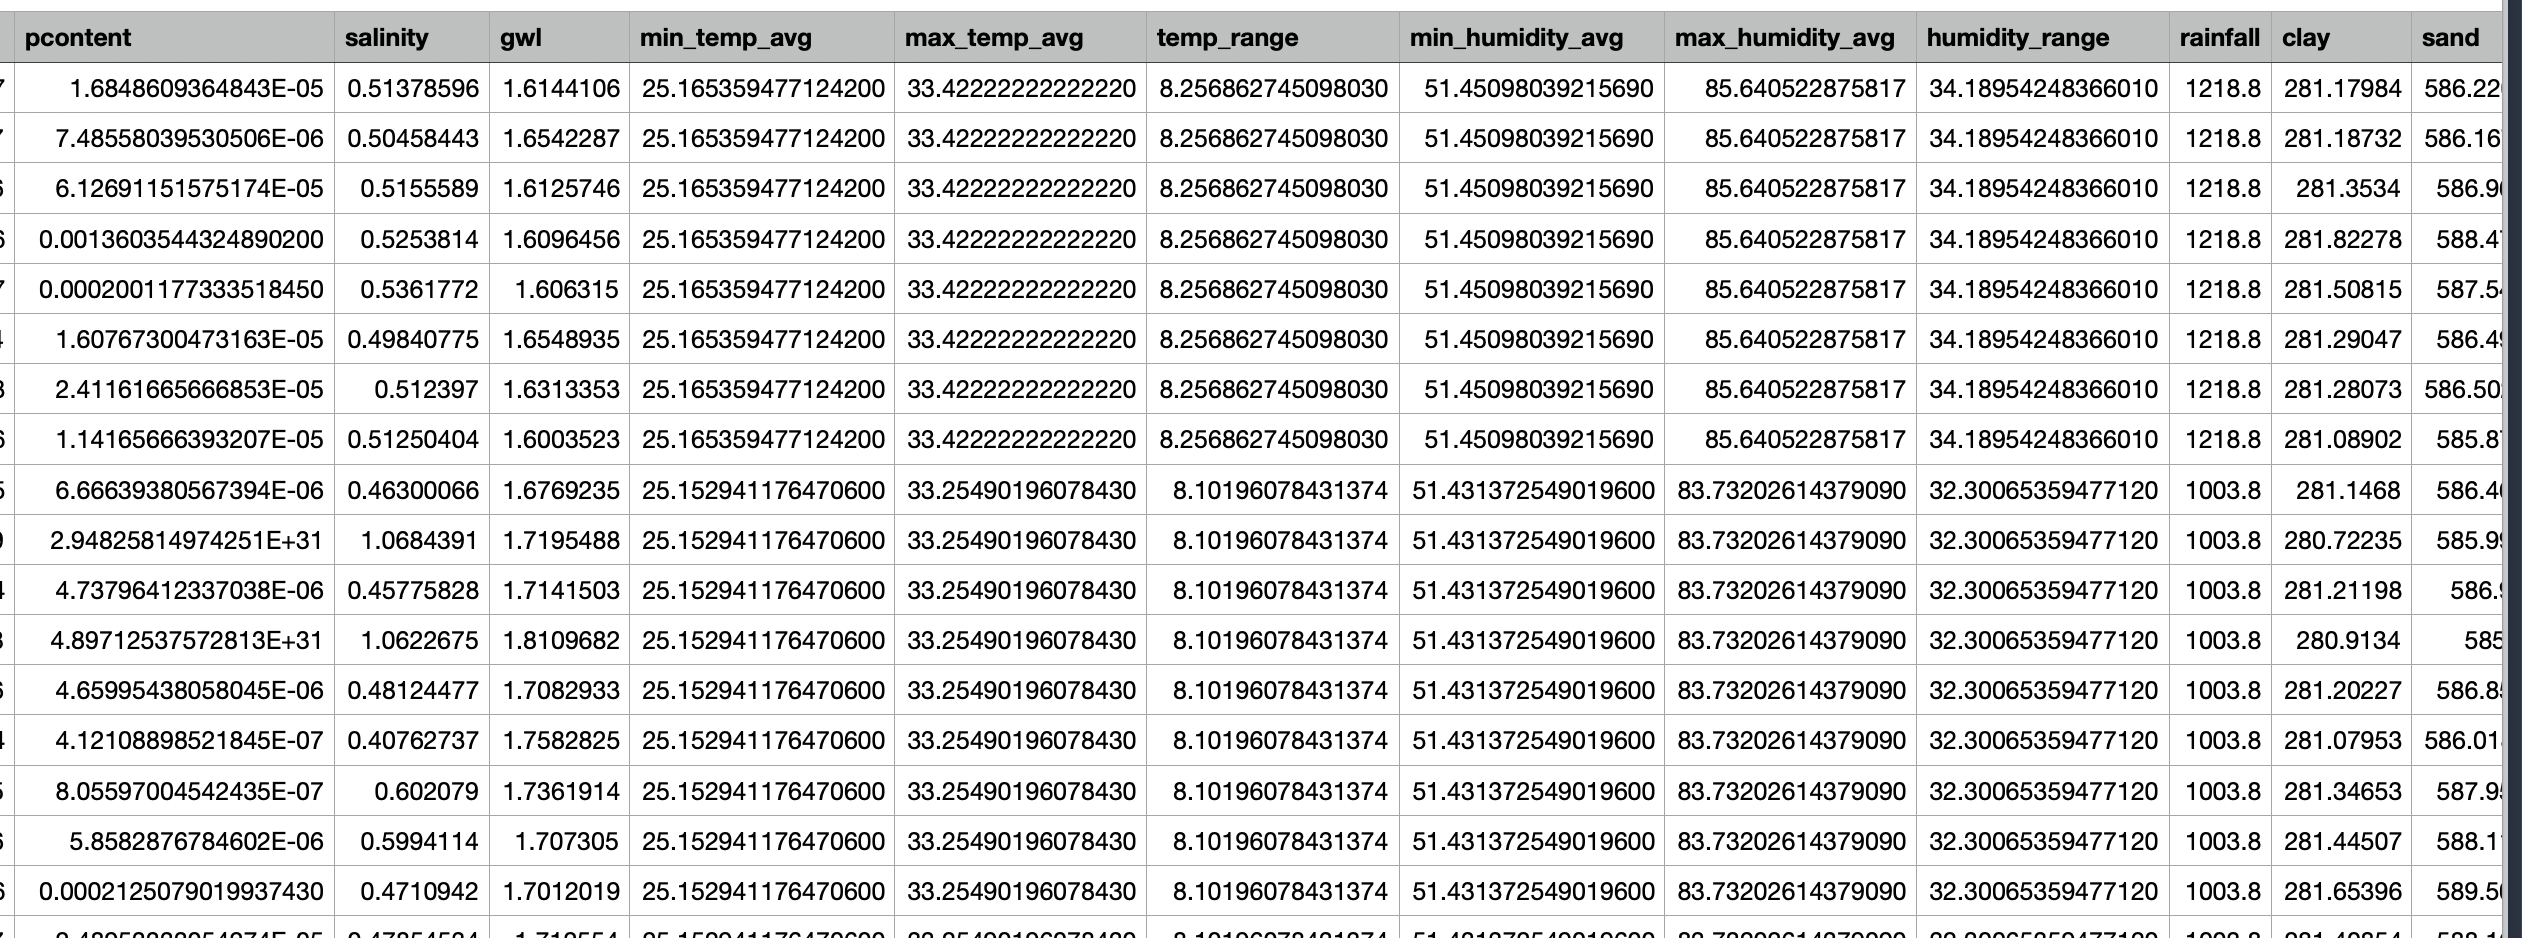
\includegraphics[width=\textwidth]{rabi_dataset.png}  % Replace with your image file
        \caption{Rabi Dataset}
    \end{minipage}
\end{frame}


% \begin{frame}{Dataset Used}
% \begin{itemize}
%     \item Dataset is prepared using Landsat-8/9 bands data and reliable government sources. There are separate dataset for both rabi and kharif seasons.
%     \item Both the Rabi and Kharif datasets contain 41 columns. These include a mix of location details, location-based characteristics, and soil characteristics derived from image data.
%     \item Each dataset has 10 band columns, which store digital numbers. These are used to compute image-based soil features. Additionally, both datasets contain 20 derived features and 8 mean reflectance values, which serve as key inputs for the model.
%     \item The last column in each dataset is the label, representing the crop cultivated in that specific district.
%     \item The Rabi dataset includes 13 different crops and has 52,127 rows. The Kharif dataset consists of 16 crops and contains 71,119 rows.
% \end{itemize}
    
% \end{frame}


% \begin{frame}{Dataset Used: Training data layout I}
% \begin{figure}
%     \centering
%     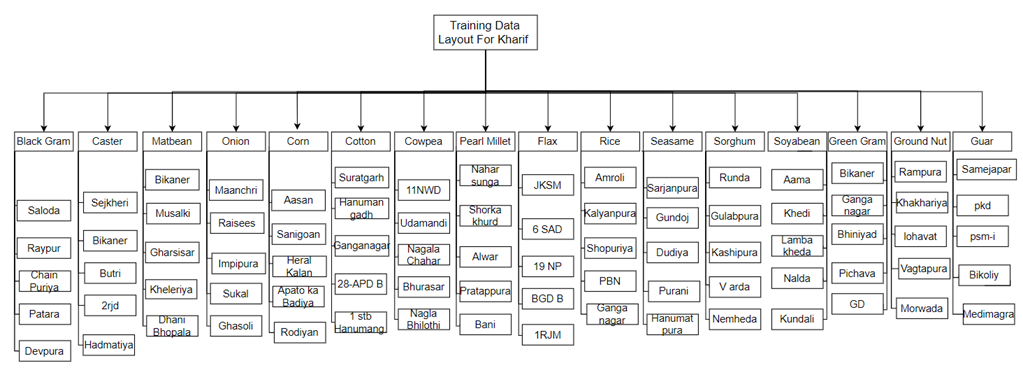
\includegraphics[width=0.80\linewidth]{images/kharif_training_layout.png}
%     \caption{For Kharif season}
%     \label{fig:enter-label}
% \end{figure}
    
% \end{frame}
% \begin{frame}{Dataset Used: Training data layout II}
% \begin{figure}
%     \centering
%     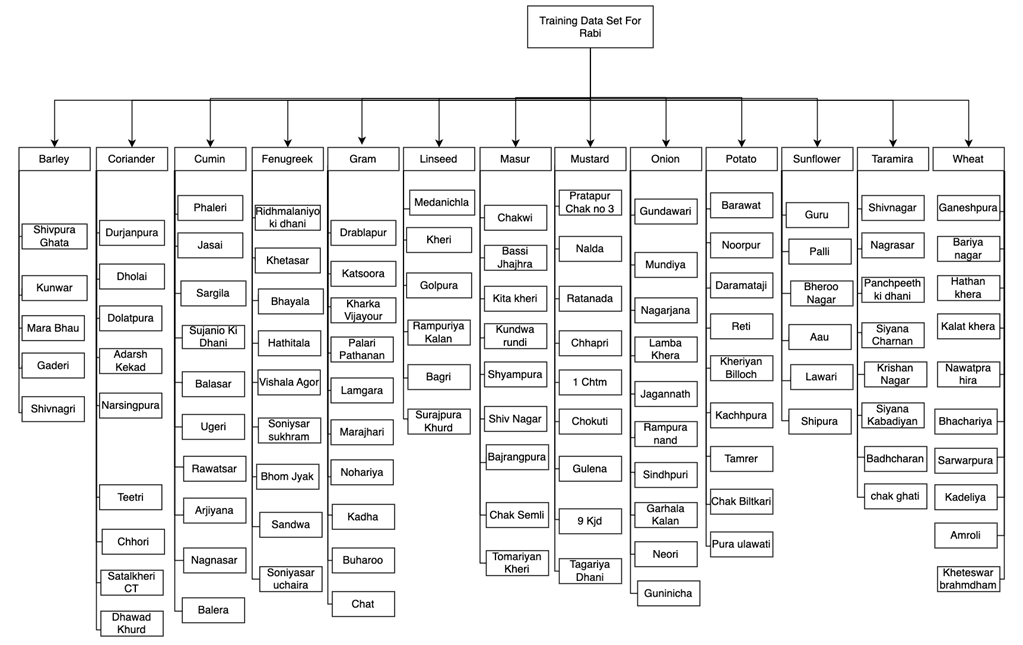
\includegraphics[width=0.68\linewidth]{images/rabi_training_layout.png}
%     \caption{For Rabi season}
%     \label{fig:enter-label}
% \end{figure}
    
% \end{frame}

% \begin{frame}{Final Dataset Produced}
%     \begin{minipage}{0.48\textwidth}
%         \centering
%         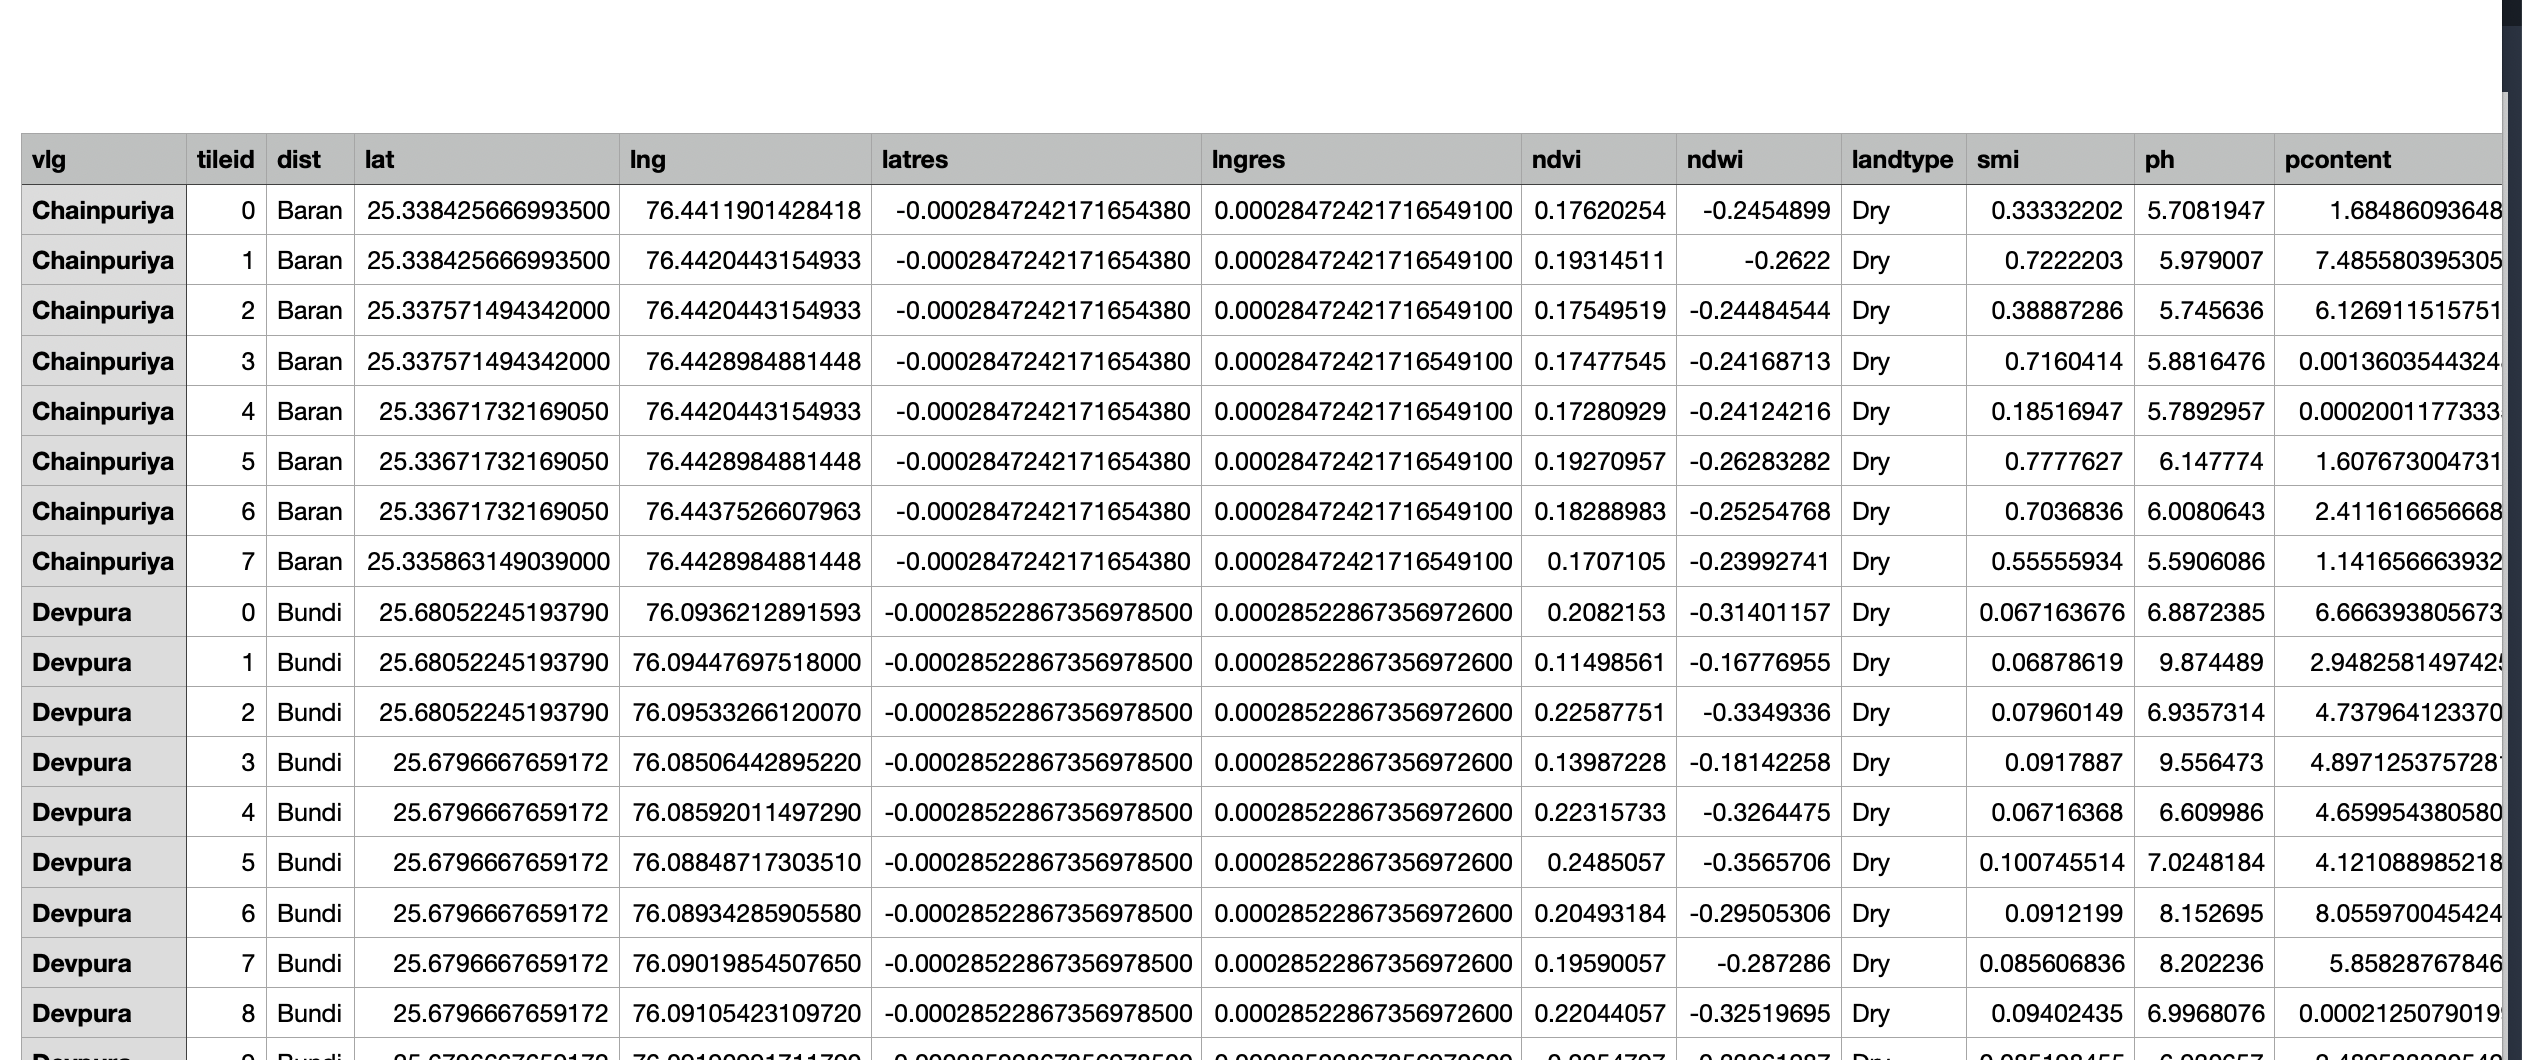
\includegraphics[width=\textwidth]{kharif_dataset.png}  % Replace with your image file
%         \caption{Kharif Dataset}
%     \end{minipage}
%     \hfill
%     \begin{minipage}{0.48\textwidth}
%         \centering
%         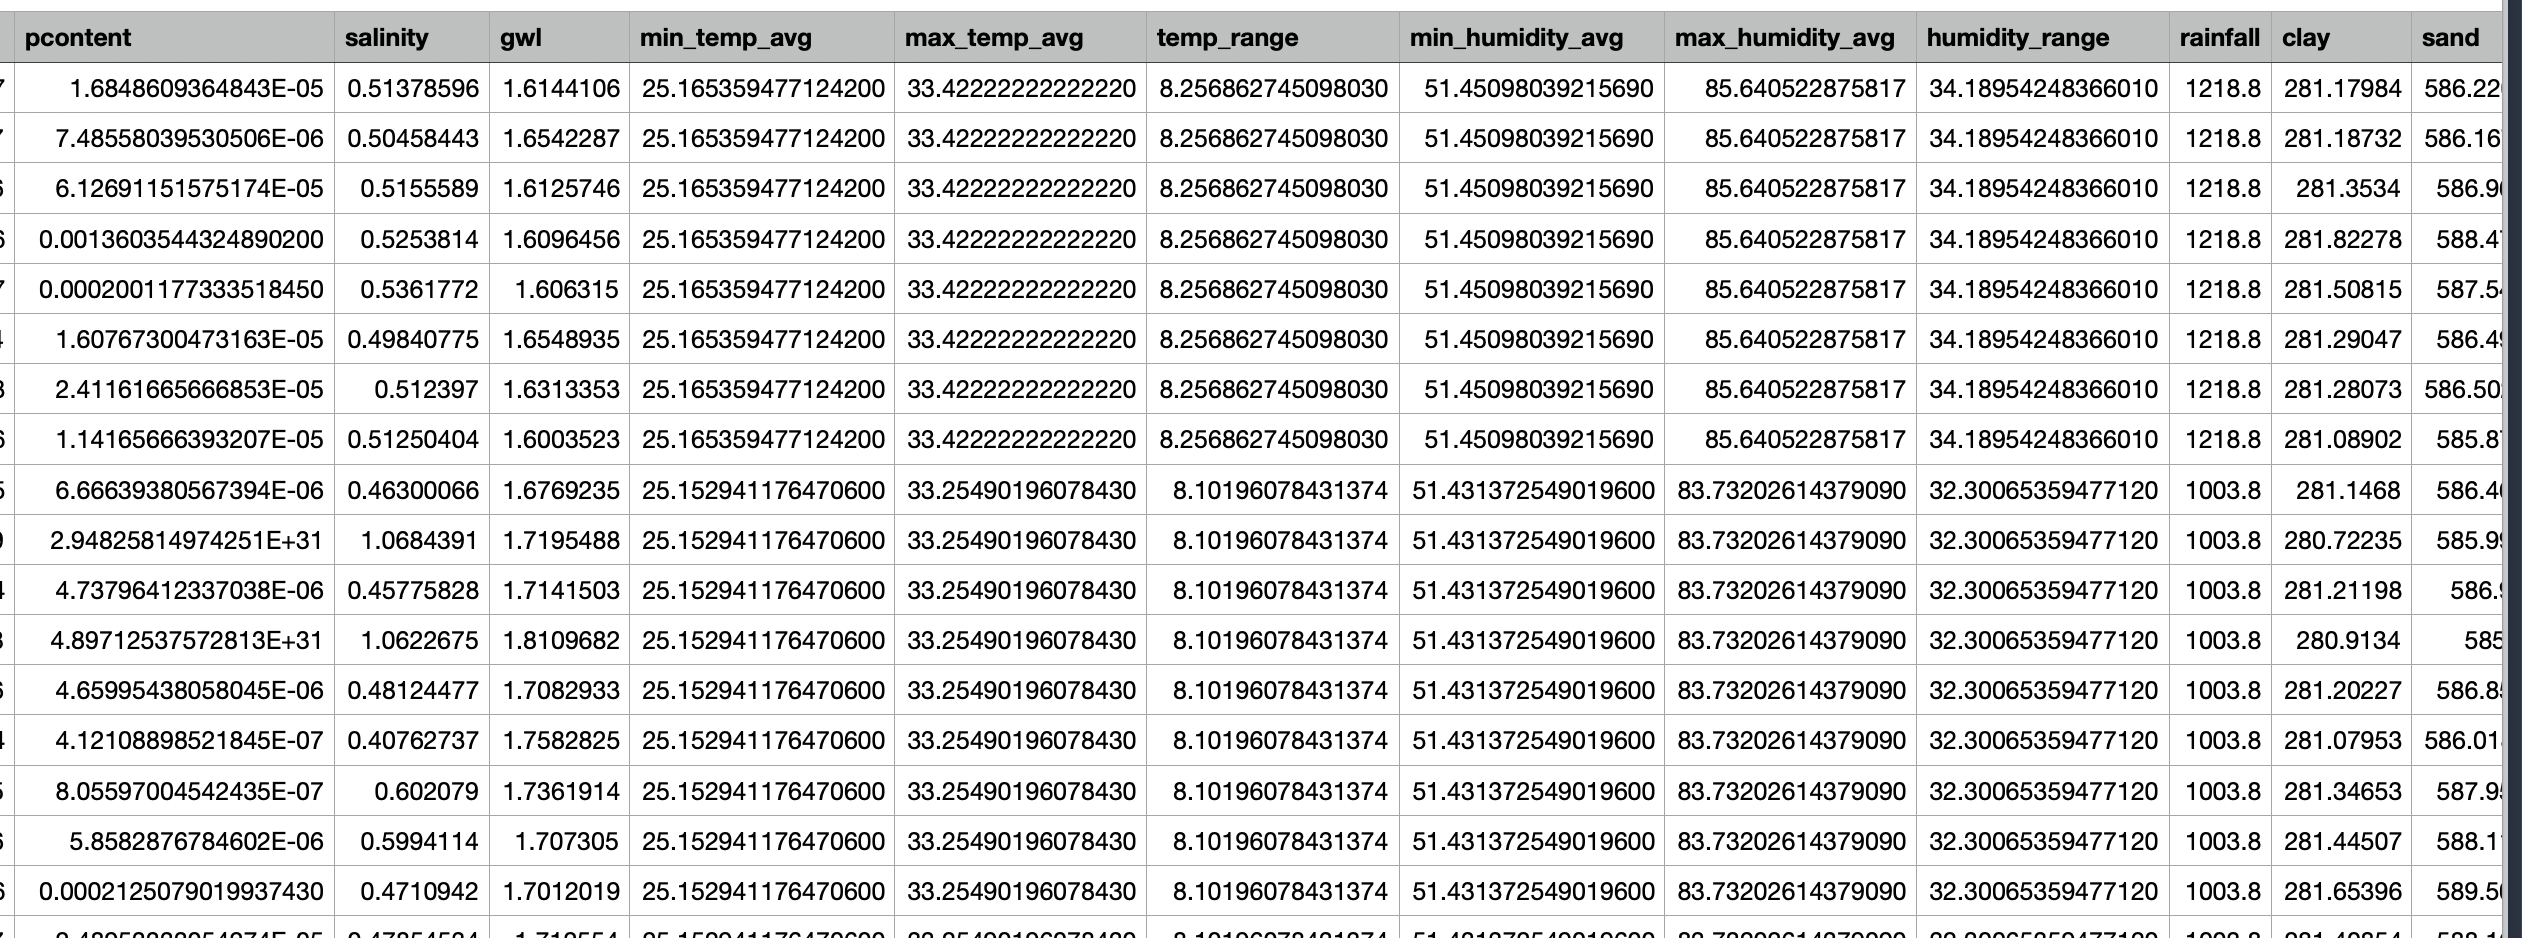
\includegraphics[width=\textwidth]{rabi_dataset.png}  % Replace with your image file
%         \caption{Rabi Dataset}
%     \end{minipage}
% \end{frame}

\begin{frame}{Layer 3: ML Algorithms Implementation Layer}
\small
    The following machine learning classifiers such as Random Forest Classifier, SVM Classifier, Decision Tree Classifier, Gradient Boosting Classifier, K Nearest Neighbor Classifier, Naïve Bayes Classifier, Logistic Regression Classifier, Artificial Neural Network and Convolutional Neural Network were used to train models over the crop dataset.

    \begin{figure}
        \centering
        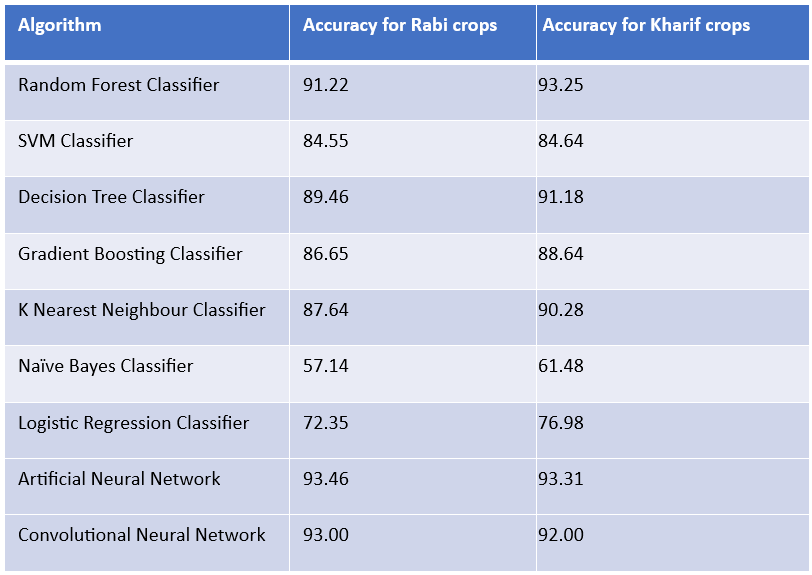
\includegraphics[scale=0.3]{images/results_ML.png}
        \caption{Accuracy comparison with different ML techniques}
        \label{fig:placeholder}
    \end{figure}
\end{frame}

% \begin{frame}{Results and Analysis}
%     \begin{figure}
%         \centering
%         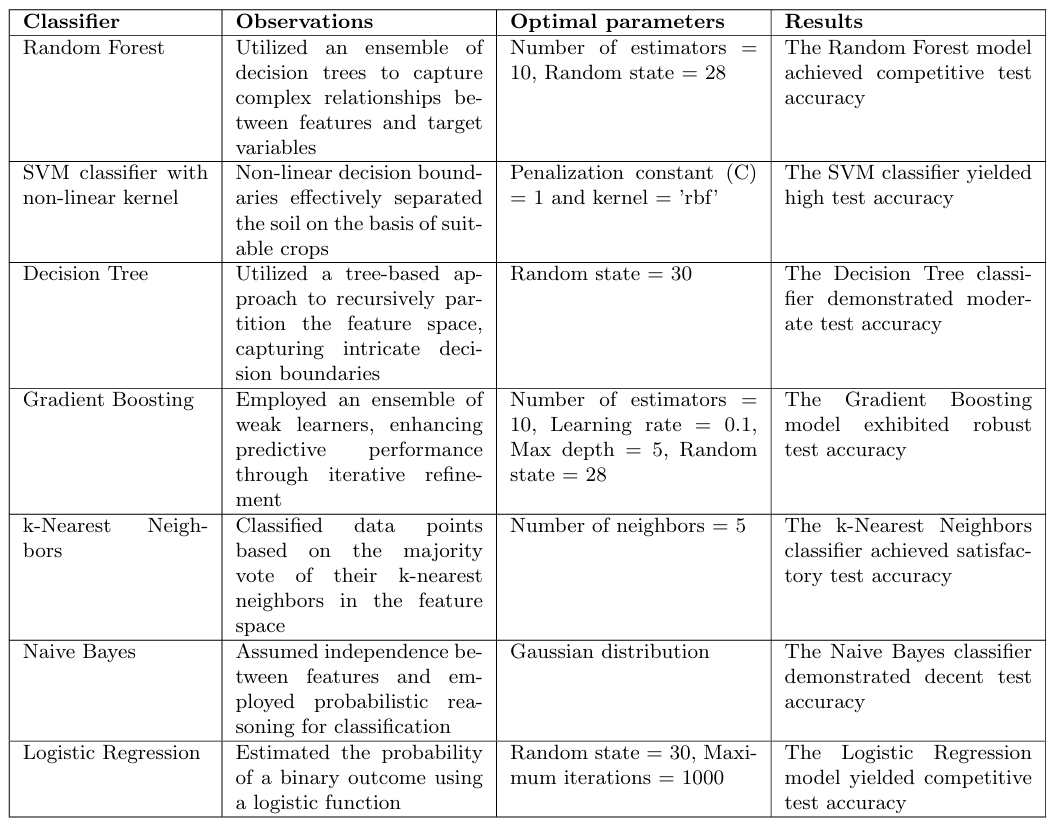
\includegraphics[width=0.6\linewidth]{images/ML_results_analysis.png}
%         \label{fig:placeholder}
%     \end{figure}
% \end{frame}

% \begin{frame}{Layer 4: ANN training and its optimization layer}
% \textbf{Nature Inspired Optimizers} \\
% Nature-Inspired Algorithms are optimization techniques that mimic natural processes and behaviors observed in biological, ecological, and physical systems to solve complex computational problems. \\
% To train the model, we will be trying various custom optimizers with ANN such as hybrids of nature inspired optimizers like PSO-SMO, BBO-EE/DOX, EEFO-CPO, etc.
% \end{frame}

% \begin{frame}{Hybrid Models I}
%     \begin{itemize}

%     \item \textbf{Hybrid ANN with PSO–SMO}
%     \begin{itemize}
%         \item Two-stage optimization: PSO for feature selection, SMO for ANN weight tuning.
%         \item Balances exploration–exploitation for complex agro-climatic datasets.
%         \item Improved accuracy for Rabi/Kharif crop datasets with scalable time complexity \(O(M \times N \times P)\).
%     \end{itemize}

%     \item \textbf{Hybrid ANN with BBO–EE/DOX}
%     \begin{itemize}
%         \item Uses growth/decline rates instead of linear immigration–emigration.
%         \item Orthogonal crossover + DPSR improves robustness and stability.
%         \item Handles imbalanced crop data and preserves solution diversity.
%     \end{itemize}

%     \item \textbf{Hybrid ANN with EEFO–CPO}
%     \begin{itemize}
%         \item Combines electric eel foraging (EEFO) and crested porcupine optimization (CPO).
%         \item Dynamic search strategy helps escape local optima.
%         \item Performs well for overlapping crop features across seasons.
%     \end{itemize}

% \end{itemize}
% \end{frame}

% \begin{frame}{Hybrid Models II}
% \begin{itemize}
% \item \textbf{Hybrid ANN with Walrus–Hippopotamus Optimizer}
%     \begin{itemize}
%         \item WOA provides global exploration; HO ensures strong exploitation.
%         \item Adaptive bounds and exploration factor guide phase switching.
%         \item Models location-specific environmental variables (NDVI, LST, NDWI, pH, salinity).
%     \end{itemize}

%     \item \textbf{Hybrid ANN with GSA–HGS}
%     \begin{itemize}
%         \item GSA enables global search via gravitational interactions.
%         \item HGS simulates survival behavior for fine-grained exploitation.
%         \item Learns long-range dependencies among soil–climate variables.
%     \end{itemize}

%     \item \textbf{Hybrid ANN with iEACOP–BBO}
%     \begin{itemize}
%         \item Combines evolutionary search (iEACOP) with migration-based exploration (BBO).
%         \item Island-model ensures parallel subpopulation evolution.
%         \item Strong at handling many spectral/environmental features simultaneously.
%     \end{itemize}

%     \item \textbf{Hybrid ANN with GSA–ALO}
%     \begin{itemize}
%         \item GSA enables diverse global exploration; ALO performs focused local hunting.
%         \item Quantum tunneling helps escape local optima.
%         \item Excellent for nonlinear soil-climate interactions (pH, P, NDVI, etc.).
%     \end{itemize}
% \end{itemize}
    
% \end{frame}

% \begin{frame}{Results}
% \begin{figure}
%     \centering
%     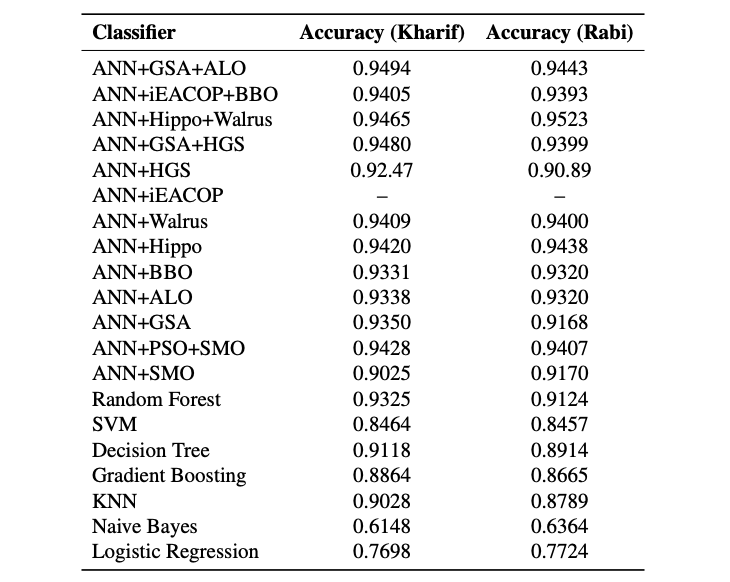
\includegraphics[width=0.4\linewidth]{images/results.png}
%     \caption{Comparison of Classifiers by Accuracy for Kharif and Rabi Datasets}
%     \label{fig:results}
% \end{figure}
% \vspace{-2mm}
% \small
% These results highlight that integrating advanced optimization techniques enhances model reliability for intelligent and scalable agricultural decision-making.

% \end{frame}

% \begin{frame}{Layer 5: Graphical User Interface}
%     \begin{figure}
%         \centering
%         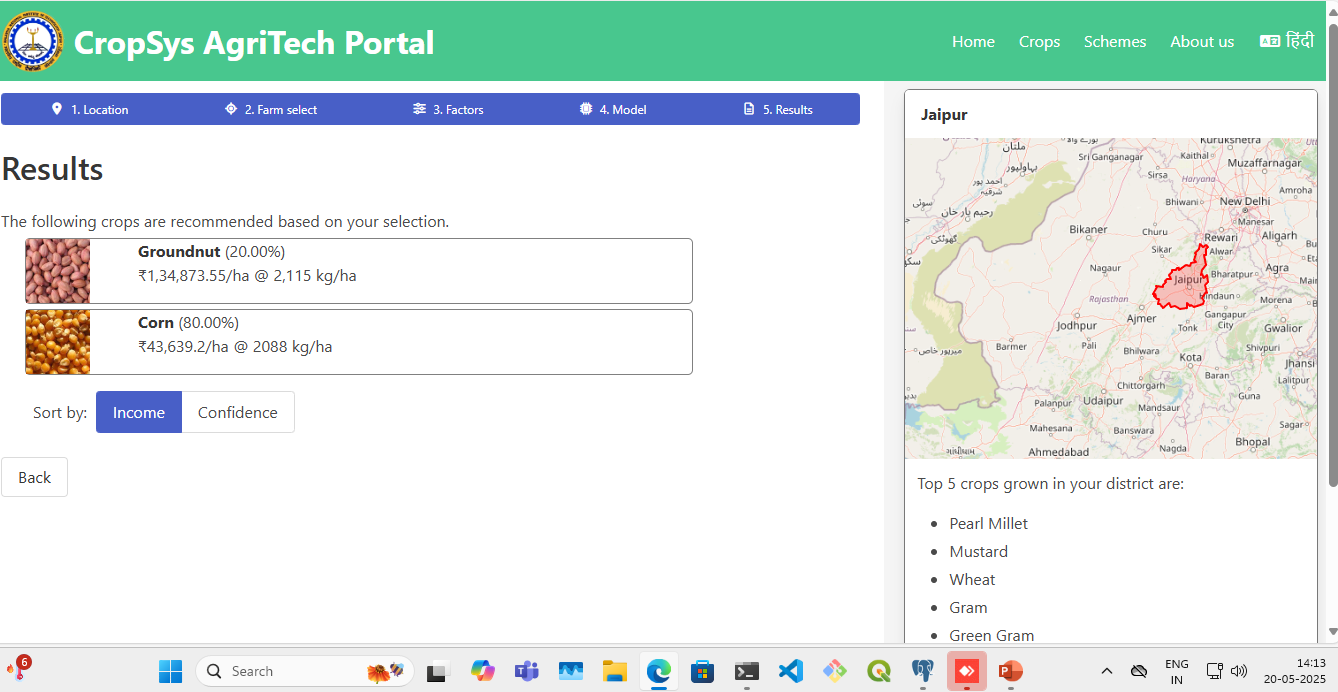
\includegraphics[width=0.75\linewidth]{images/gui_3.png}
%         \caption{Recommended crops based on user inputs}
%         \label{fig:enter-label}
%     \end{figure}
% \end{frame}

\begin{frame}{GUI for Crop Recommendation System}
The existing portal is shown below.
\begin{figure}
    \centering
    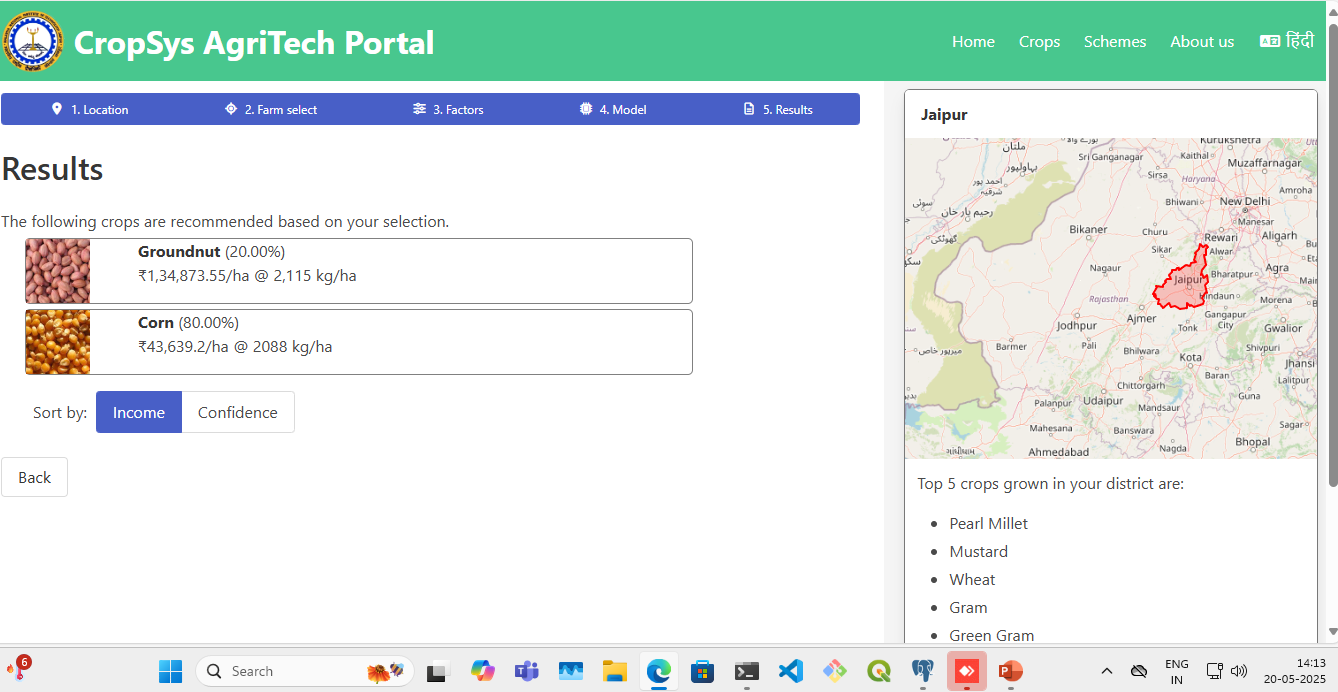
\includegraphics[width=0.5\linewidth]{images/gui_3.png}
    \caption{Graphical User Interface for Existing CRS}
    \label{fig:placeholder}
\end{figure}
We plan to integrate a richer temporal dataset and newer models on this portal.
    
\end{frame}

\begin{frame}{Ongoing Work}
\begin{itemize}
    \item Downloaded and pre-processed \textbf{Landsat 8/9 datasets} and \textbf{Dynamic World crop-masks} for 2022–23 and 2023–24 to expand beyond the current 2021–22 training year.
    
    \item In active coordination with the \textbf{Rajasthan Statistics Department} for retrieval of updated village-level area-under-cultivation data.
    
    \item Collected \textbf{weather, soil, and knowledge-based features} (rainfall, temperature, humidity, soil moisture, spectral indices) to enrich the multi-year dataset.
    
    \item Conducting an extensive \textbf{study of latest Nature-Inspired Algorithms (2025)} to identify strong candidates for integration with existing ANN models for further performance enhancement.
    
\end{itemize}
\end{frame}

\begin{frame}{Conclusion \& Future Scope}
\small
The study successfully reconstructed the original crop recommendation dataset by integrating village-level agricultural records, Landsat 8/9 satellite imagery, weather parameters, and soil-based derived features. This high-resolution, multi-feature dataset enabled the evaluation of baseline classification models such as KNN, Decision Trees, Random Forests, and SVM. Experimental results showed that while these traditional models perform reasonably well on curated data, their accuracy remains limited by temporal gaps, high feature dimensionality, and non-linear agro-climatic patterns. These findings highlight the importance of a multi-year dataset and advanced optimization-driven learning frameworks.

\vspace{5mm}

\textbf{Future Work:}
\begin{itemize}
    \item Train the enhanced models on a \textbf{comprehensive multi-year dataset} (2021–22 to 2023–24) capturing climatic, soil, spectral, and spatial variability.
    \item Develop a \textbf{hybrid deep learning model} integrated with the latest NIAs for highly accurate multi-crop classification and crop recommendation.
\end{itemize}

\end{frame}

\begin{frame}{Acknowledgements}
    \begin{itemize}
        \item As a part of this project, we would like to express our sincere gratitude to the Department of Science and Technology, Anusandhan National Research Foundation (ANRF/SERB) under the Core Research Grant Scheme (File no. DST/CRG/2022/000472 and sanction order ANRF/F/8568/2024-2025) for giving financial support at the Department of Computer Science and Engineering, Malaviya National Institute of Technology, Jaipur, India. 
        \item We also thank Mr. Gopal Lal Morrya (Statistical Officer, TRS \& Agriculture), Department of Statistics, Govt. Of Rajasthan for supplying village-level agricultural data and for their valuable cooperation throughout this work.
    \end{itemize}
\end{frame}

% \begin{frame}[plain]
%     \vfill
%     \begin{center}
%         
\includegraphics[scale=1]{images/thank you.jpg}
%     \end{center}
%     \vfill
% \end{frame}

% \begin{frame}{References}
% \scriptsize
%     \printbibliography
% \end{frame}


\end{document}